\section{Theorie}
\label{sec:Theorie}
\subsection{Ziel}
Ziel des Versuchs 351 ist die Untersuchung von RC-Gliedern.
 Dabei werden Zeitkonstante, Frequenzabhängikeit von Amplitude und Phasenverschiebung bestimmt, sowie die Eignung als Integrator betrachtet.
\subsection{Ent- und Aufladevorgang eines Kondensators}
Als Relaxationserscheinung wird die nicht-oszillatorische Rückkehr eines Systems in seinen Ausgangszustand bezeichnet, welches zuvor aus diesem rausgenommen wird.
Ein Beispiel für einen Relaxationsvorgang dient der Ent- und Aufladevorgang eines Kondensators über einen Widerstand.
Auf den Platten eines Kondensators befindet sich die Ladung Q, somit gilt für die Spannung zwischen den Platten:\\
\begin{equation}
  U_C=\frac{Q}{C}.
\end{equation}\\
Mit dem ohmschen Gesetzt ergibt sich ein Strom:\\
\begin{equation}
  I=\frac{U_C}{R}.
\end{equation}\\
Ebenfalls gilt die Beziehung
\begin{equation}
  \dot Q= -I.
\end{equation}\\
Diese Beziehungen führen zu der Differentialgleichung:
\begin{equation}
  \dot Q= -\frac{1}{RC}  Q(t).
\end{equation}\\
Es greift die Annahme, dass der Kondensator sich nach unendlich langer Zeit entladen hat, somit gilt $Q(\infty)=0$. Mit weiterer Integration folgt:
\begin{equation}
  Q(t)=Q(0)e^{-\frac{t}{RC}}\label{eqn:entladung}
\end{equation}
hierbei wird RC als Zeitkonstante bezeichnet, diese gibt das Maß für die Geschwindigkeit an, mit welcher das System in den Zustand $Q(\infty)$ strebt.\\
Für den Aufladevorgang gelten analoge Annahmen, sodass sich, mit den Randbedingungen $Q(0)=0$ und $Q(\infty)=CU_0$, eine Gleichung für den Aufladevorgang ableiten lässt:
\begin{equation}
  Q(t)=CU_0(1-e^{-\frac{t}{RC}}).\label{eqn:aufladung}
  \end{equation}
  $U_0$ beschreibt die anliegende Spannung einer Spannungsquelle.
\subsection{Frequenzabhängigkeit von Phasenverschiebung und Amplitude}
Relaxationsvorgänge treten auch in Systemen auf, die periodisch aus der Ausgangslage ausgelenkt werden.
Mit der Verwendung einer Wechselspannung als anliegende Spannung, kann der RC-Kreis weiterhin als ein Beispiel verwendet werden, wie in Abbildung zu sehen.\\ %Abbildung 2
\begin{figure}
  \centering
  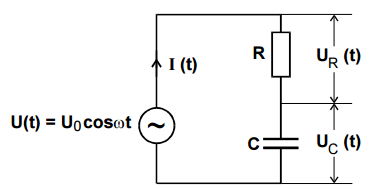
\includegraphics[width=0.7\textwidth]{schaltbild2.PNG}
  \caption{Schaltungsbeispiel.\cite{skript}}
  \label{fig:schaltung2}
\end{figure}\\
Gilt für $\omega$, in der Wechselspannung $U(t)=U_0\cos\omega t$, die Beziehung $\omega\textless\textless\frac{1}{RC}$
so sind $U_C(t)$ und $U(t)$ zu jedem Zeitpunk fast gleich.
Mit größerer Frequenz ergibt sich eine immer größer werdende Phasenverschiebung $\phi$ zwischen der Generator-und Kondensatorspannung,
ebenfalls nimmt die Amplitude der Kondensatorspannung ab.\\
Für den allgemeinen RC-Kreis gilt mit dem Ansatz $U_C(t)=A(\omega)\cos(\omega t+\phi{\omega})$,
der zweiten Kirchhoffschen Regel und einigen Umformungen:
\begin{equation}
  U_0\cos\omega t =-A\omega RC\sin(\omega t+\phi)+A(\omega)\cos(\omega t+\phi).\label{eqn:RCallgemein}
\end{equation}\\
Diese Gleichung ist für alle t gültig.
Es ergibt sich eine frequenzabhängige Beziehung für die Phasenverschiebung:
\begin{equation}
  \phi(\omega)=\arctan(-\omega RC)
\end{equation}
Ebenfalls lässt sich aus der Gleichung \eqref{eqn:RCallgemein} eine frequenzabhängige Beziehung für die Amplitude der Kondensatorspannung ableiten:
\begin{equation}
  A(\omega)=\frac{U_0}{\sqrt{1+\omega^{2}R^2c^2}}.\label{eqn:amplitude}
\end{equation}
$A(\omega)$ geht gegen $U_0$ für $\omega\longrightarrow 0$ und verschwindet bei $\omega\longrightarrow\infty$.
\subsection{Eigenschaft als Integrator}
Ein RC-Kreis kann Wechselspannungen $U_t$ mit Frequenzen größer als $\frac{1}{RC}$ integrieren.
Unter dieser Bedingung ergibt sich folgendes Integral:
\begin{equation}
  U_C(t)=\frac{1}{RC}\int_{0}^{1} U(t') \, \symup{d}t.'\label{eqn:integration}
\end{equation}
